%%%%%%%%%%%%%%%%%%%%%%%%%%%%%%%%%%%%%%%%%
% Beamer Presentation
% LaTeX Template
% Version 1.0 (10/11/12)
%
% This template has been downloaded from:
% http://www.LaTeXTemplates.com
%
% License:
% CC BY-NC-SA 3.0 (http://creativecommons.org/licenses/by-nc-sa/3.0/)
%
%%%%%%%%%%%%%%%%%%%%%%%%%%%%%%%%%%%%%%%%%

%----------------------------------------------------------------------------------------
%	PACKAGES AND THEMES
%----------------------------------------------------------------------------------------
%dont fuck with this
\documentclass{beamer}
\setbeamertemplate{background} 
{
\includegraphics[width=\paperwidth,height=\paperheight]{background.jpg}}

\mode<presentation> {

% The Beamer class comes with a number of default slide themes
% which change the colors and layouts of slides. Below this is a list
% of all the themes, uncomment each in turn to see what they look like.
\usepackage{hyperref}
%\usetheme{default}
%\usetheme{AnnArbor}
%\usetheme{Antibes}
%\usetheme{Bergen}
%\usetheme{Berkeley}
%\usetheme{Berlin}
%\usetheme{Boadilla}
%usetheme{CambridgeUS}
%\usetheme{Copenhagen}
%\usetheme{Darmstadt}
%\usetheme{Dresden}
%\usetheme{Frankfurt}
%\usetheme{Goettingen}
%\usetheme{Hannover}
%\usetheme{Ilmenau}
%\usetheme{JuanLesPins}
%\usetheme{Luebeck}
%\usetheme{Madrid}
%\usetheme{Malmoe}
%\usetheme{Marburg}
%\usetheme{Montpellier}
%\usetheme{PaloAlto}
%\usetheme{Pittsburgh}
%\usetheme{Rochester}
%\usetheme{Singapore}
%\usetheme{Szeged}
\usetheme{Warsaw}

% As well as themes, the Beamer class has a number of color themes
% for any slide theme. Uncomment each of these in turn to see how it
% changes the colors of your current slide theme.

\usecolortheme{albatross}
%\usecolortheme{beaver}
%\usecolortheme{beetle}
%\usecolortheme{crane}
%\usecolortheme{dolphin}
%\usecolortheme{dove}
%\usecolortheme{fly}
%\usecolortheme{lily}
%\usecolortheme{orchid}
%\usecolortheme{rose}
%\usecolortheme{seagull}
%\usecolortheme{seahorse}
%\usecolortheme{whale}
%\usecolortheme{wolverine}

%\setbeamertemplate{footline} % To remove the footer line in all slides uncomment this line
%\setbeamertemplate{footline}[page number] % To replace the footer line in all slides with a simple slide count uncomment this line

%\setbeamertemplate{navigation symbols}{} % To remove the navigation symbols from the bottom of all slides uncomment this line
}
\usepackage{media9}
\usepackage{graphicx} % Allows including images
\usepackage{booktabs} % Allows the use of \toprule, \midrule and \bottomrule in tables
\usepackage{cite}
 \usepackage{multimedia}
\setbeamertemplate{navigation symbols}{}
\setbeamertemplate{bibliography item}{\insertbiblabel}
\setbeamertemplate{frametitle continuation}[from second]
%----------------------------------------------------------------------------------------
%	TITLE PAGE
%----------------------------------------------------------------------------------------

\title[] { Continuous integration pipeline implementation for Tech11 software
}
\author[]{By\\ Aswin G Sugunan(13)\\Jeffin Jacob(17)\\Nitin Suresh(25)\\Vishnu Bose(39)\\Guided By\\Mrs.Greeshma\\Asst.Professor in CSE}
\institute[CE CHERTHALA]{COLLEGE OF ENGINEERING CHERTHALA}
\date{\today}
%\date{8/8/16} % Date, can be changed to a custom date

\begin{document}

\begin{frame}
\titlepage % Print the title page as the first slide
\end{frame}

\begin{frame}
\frametitle{Overview} % Table of contents slide, comment this block out to remove it
\tableofcontents % Throughout your presentation, if you choose to use \section{} and \subsection{} commands, these will automatically be printed on this slide as an overview of your presentation
\end{frame}

%----------------------------------------------------------------------------------------
%	PRESENTATION SLIDES
%----------------------------------------------------------------------------------------
% Sections can be created in order to organize your presentation into discrete blocks, all sections and subsections are automatically printed in the table of contents as an overview of the talk
%------------------------------------------------

%\subsection{} % A subsection can be created just before a set of slides with a common theme to further break down your presentation into chunks
%\subsection{Android System}


%\begin{frame}{Title}
%
% \includemedia[
%  width=\paperwidth,
%  height=0.7\linewidth,
%   activate=onclick,
%   deactivate=onclick,
% addresource=ero.mp4,
% flashvars={source=ero.mp4
% &loop=false
% &scaleMode=letterbox
%    }
% ]{\textsc{0.02in}{erotion}}{VPlayer.swf}
 

 
% \begin{center}
%\href{run:/usr/local/bin/mplayer -fs forced_pendulum.mp4}{
%\includegraphics[scale=0.25]
%{forced_pendulum.eps}}
%\end{center}
% \end{frame}
\section{INTRODUCTION}
\begin{frame}{(Common) Scenario}
%\begin{itemize}
%\item 
\begin{itemize}
\item \textbf {Developers working on a project.}
\begin{itemize}
\vspace{10pt}
\item They each implement a few class.
\begin{itemize}
\vspace{10pt}
\item Code them.
\vspace{10pt}
\item Ensure well tested.
\end{itemize}
\vspace{10pt}
\item When they're done,They \textit{integrate} them.
\begin{itemize}
\vspace{10pt}
\item Every thing breaks.
\end{itemize}
\end{itemize}
\end{itemize}


% \item

%\begin{figure}
%\begin{center}
%\includegraphics[scale=0.5]{scene1.jpg}
%\caption{Scene Character }
%\end{center}
%\end{figure}


%\end{itemize}
\end{frame}
\begin{frame}{Integration Hell}
\begin{quote}
\textbf{That awkward moment near the end of the project when everyone realizes that none of their classes interoperate correctly.}
\end{quote} 
\end{frame}
\begin{frame}{Integration Hell (cont..)}
\textbf{Integration hell is extremely risk for a project.}
\begin{itemize}
\vspace{10pt}
\item \textbf{Difficult to determine how long it will take to resolve the integration process.}
\begin{itemize}
\vspace{10pt}
\item May (vastly) exceed our budget.
\vspace{10pt}
\item May (vastly )exceed our schedule.
\end{itemize}
\end{itemize}
\end{frame}

\section{PROPOSED SYSTEM}  

\begin{frame}{Continues Integration}
\vspace{0.5cm}
 \begin{itemize}
\item \textbf{Originated from eXtreme Programing (XP).}
\vspace{.5 cm}
\item \textbf{Mitigates risk associated with integrating Software.} 
\vspace{.5 cm}
\item\textbf{Avoids integration hell.}

\vspace{.5 cm}
\item \textbf{Integrate \textit{early} and integrate \textit{often}.}
\vspace{.5 cm}
 \begin{itemize}
\item \textit{ie}, on every change.
\end{itemize}
\end{itemize}
\end{frame}  

\begin{frame}{Evolution of software delivery}
	\begin{itemize}
		\item Waterfall 
		\item Agile
		\item Continuous Delivery
		\begin{itemize}
			\item Another subset of agile which in which the team keeps its software ready for release at all times during development. It is different from “traditional” agile in that it does not involve stopping and making a special effort to create a releasable build.
		\end{itemize}
		\end{itemize}
\end{frame}

\begin{frame}{Continues Integration}

 \textbf {Automates the process of building,testing,reporting.}
\begin{figure}
\begin{center}
\includegraphics[scale=2.5]{hudson1.jpg}
\end{center}
\end{figure}
\end{frame}

\begin{frame}{Benefits of CI server}
\vspace{0.5cm}
 \begin{itemize}
\item \textbf{Developer might forget to run the test.}
\begin{itemize}
\vspace{0.5cm}
\item \textit{Don't break the build.}
\end{itemize}
\vspace{0.5cm}
\item \textbf{It may take too long to run the tests.}
\vspace{0.5cm}
\item \textbf{We might need to test the code in various environments.} 
\vspace{0.5cm}
\begin{itemize}
\item Different architectures (32-bit,64-bit,ARM,PowerPC).
\vspace{0.5cm}
\item Different platforms (Windows,Linux,Mac,Solaris).
\end{itemize}
\end{itemize}
\end{frame} 

\begin{frame}{Benefits of CI server (cont..)}
\vspace{0.5cm}
 \begin{itemize}
\item \textbf{Reports provide useful insights to team.}
\begin{itemize}
\vspace{0.5cm}
\item Can track metrics like line coverage.
\begin{itemize}
\vspace{0.5cm}
\item Percentage of line executed by a program's test.
\end{itemize}
\end{itemize}
\begin{itemize}
\vspace{0.5cm}
\item Can run all sorts of utilities on our code.
\begin{itemize}
\vspace{0.5cm}
\item \textit{CheckStyle, Findbugs, ..}
\end{itemize}
\end{itemize}
\item \textbf{Can deploy automatically.}
\vspace{0.5cm}
\begin{itemize}
\item Deploy a web project to a stagging server.
\vspace{0.5cm}
\item Deploy latest stable build of a desktop application to our website for download.
\end{itemize}
\end{itemize}
\end{frame} 

\section{MODULES}
\begin{frame}{Modules}
\begin{itemize}
\item Version Control
\item Artifact Manager
\item Continuous Integration Handler
\item Test Automator

\end{itemize}

\end{frame}

\begin{frame}{Modules}
\begin{itemize}
\item \underline{Version Control}
\item Artifact Manager
\item Continuous Integration Handler
\item Test Automator

\end{itemize}

\end{frame}

\begin{frame}{Version Control}
\begin{itemize}
\item This practice advocates the use of a revision control system for the project’s source code.
\vspace{0.5 cm}
\item In this
practice and in the revision control community, the convention is that the system should
be buildable from a fresh checkout and not require additional dependencies.
\end{itemize}
\end{frame}


\begin{frame}{Version Control}
	\begin{itemize}
		\item Here we use Git-Hub for version controlling.
		\vspace{0.5 cm}
		\item GitHub is a web-based Git or version control repository and Internet hosting service. It offers all of the distributed version control and source code management functionality of Git as well as adding its own features.
	\end{itemize}

\includegraphics[scale=0.2]{github.png}
\end{frame}
\begin{frame}{Modules}
\begin{itemize}
\item Version Control
\item Artifact Manager
\item Continuous Integration Handler
\item Test Automator

\end{itemize}

\end{frame}

\begin{frame}{Modules}
\begin{itemize}
\item Version Control
\item \underline{Artifact Manager}
\item Continuous Integration Handler
\item Test Automator

\end{itemize}

\end{frame}

\begin{frame}{Artifact Manager}
\begin{itemize}
%\item An artifact repository is akin to what Subversion is to source code, i.e. it is a way of versioning code binary artifacts. In the Java world these artifacts could be jars, wars, ears, fully fledged applications, libraries or a collections of libraries that are packaged.
%\vspace{0.5 cm}
%\item Jenkins stores the artifacts as plain files without versioning while artifacts in an artifact repository can be version controlled.

	\item Artifact repositories are great at managing multilevel dependencies, much better then the old text file with a list that developers update and maintain. 
	\vspace{0.5 cm}
\item Critical for reducing errors and ensuring the right pieces make it with each build/deployment/release, especially in large-scale business applications.
\vspace{0.5 cm}
\item video
\end{itemize}
\end{frame}


\begin{frame}{Modules}
\begin{itemize}
\item Version Control
\item Artifact Manager
\item Continuous Integration Handler
\item Test Automator

\end{itemize}

\end{frame}

\begin{frame}{Modules}
\begin{itemize}
\item Version Control
\item Artifact Manager
\item \underline{Continuous Integration Handler}
\item Test Automator

\end{itemize}

\end{frame}

\begin{frame}{Continuous Integration Handler}
\begin{itemize}
\item  It integrates with popular build tools (ant, maven, make) so that it can run the appropriate
build scripts to compile, test and package within an environment that closely
matches what will be the production environment
\item It integrates with version control tools, including Subversion, so that different projects
can be set up depending on projection location within the trunk.
\item It can be configured to trigger builds automatically by time and/or changeset. (i.e.,
if a new changeset is detected in the Subversion repository for the project, a new
build is triggered.)
\item It reports on build status. If the build is broken, it can be configured to alert individuals
by email.
\end{itemize}
\end{frame}



\begin{frame}{Modules}
\begin{itemize}
\item Version Control
\item Artifact Manager
\item Continuous Integration Handler
\item Test Automator

\end{itemize}

\end{frame}

\begin{frame}{Modules}
\begin{itemize}
\item Version Control
\item Artifact Manager
\item Continuous Integration Handler
\item \underline{Test Automator}

\end{itemize}

\end{frame}

\begin{frame}{Test Automator}
\begin{itemize}
\item  In software testing, test automation is the use of special software (separate from the
software being tested) to control the execution of tests and the comparison of actual outcomes with predicted outcomes
\vspace{0.5 cm}
\item Test automation is critical for continuous
delivery and continuous testing.
\vspace{0.5 cm}
\begin{itemize}
\item  Graphical user interface testing.
\item API driven testing.
\end{itemize}
\end{itemize}
\end{frame}

\begin{frame}{Operating Environment}
\begin{itemize}
\item The system is expected to be operated in Linux as well as in windows with the support of
respective JRE (Java Runtime Environment). This system based project is completely platform
independent. The most important requirement is the internet connection.
\end{itemize}
\end{frame}

\begin{frame}{Gantt Chart}
\begin{figure}[h]
\begin{center}
%\epsfig{width=6in, file=gant.jpg}
\includegraphics[scale=0.28]{LogicBakerGantt.pdf}
\caption{Gantt Chart}
\end{center}
\end{figure}
\end{frame}

\begin{frame}{Data Flow Diagram}
\begin{itemize}
\item level 0
\end{itemize}
\begin{figure}[h]
\begin{center}
%\epsfig{width=6in, file=gant.jpg}
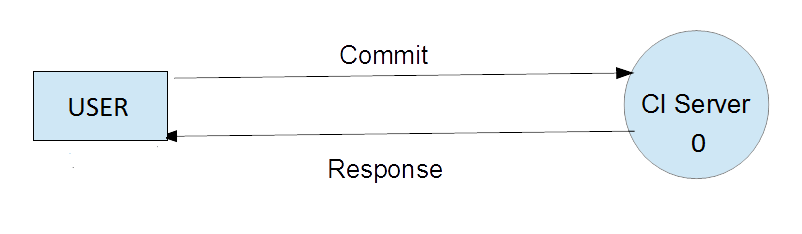
\includegraphics[scale=0.28]{dfd1.png}
\caption{level 0 dfd}
\end{center}
\end{figure}
\end{frame}

\begin{frame}{Data Flow Diagram}
\begin{itemize}
\item level 1
\end{itemize}
\begin{figure}[h]
\begin{center}
%\epsfig{width=6in, file=gant.jpg}
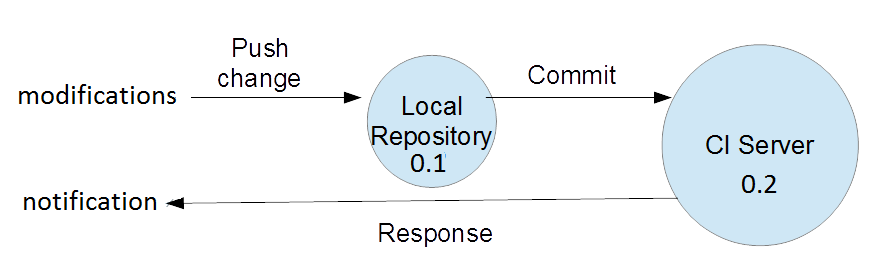
\includegraphics[scale=0.28]{dfd2.png}
\caption{level 1 dfd}
\end{center}
\end{figure}
\end{frame}

\begin{frame}{Data Flow Diagram}
\begin{itemize}
\item level 2
\end{itemize}
\begin{figure}[h]
\begin{center}
%\epsfig{width=6in, file=gant.jpg}
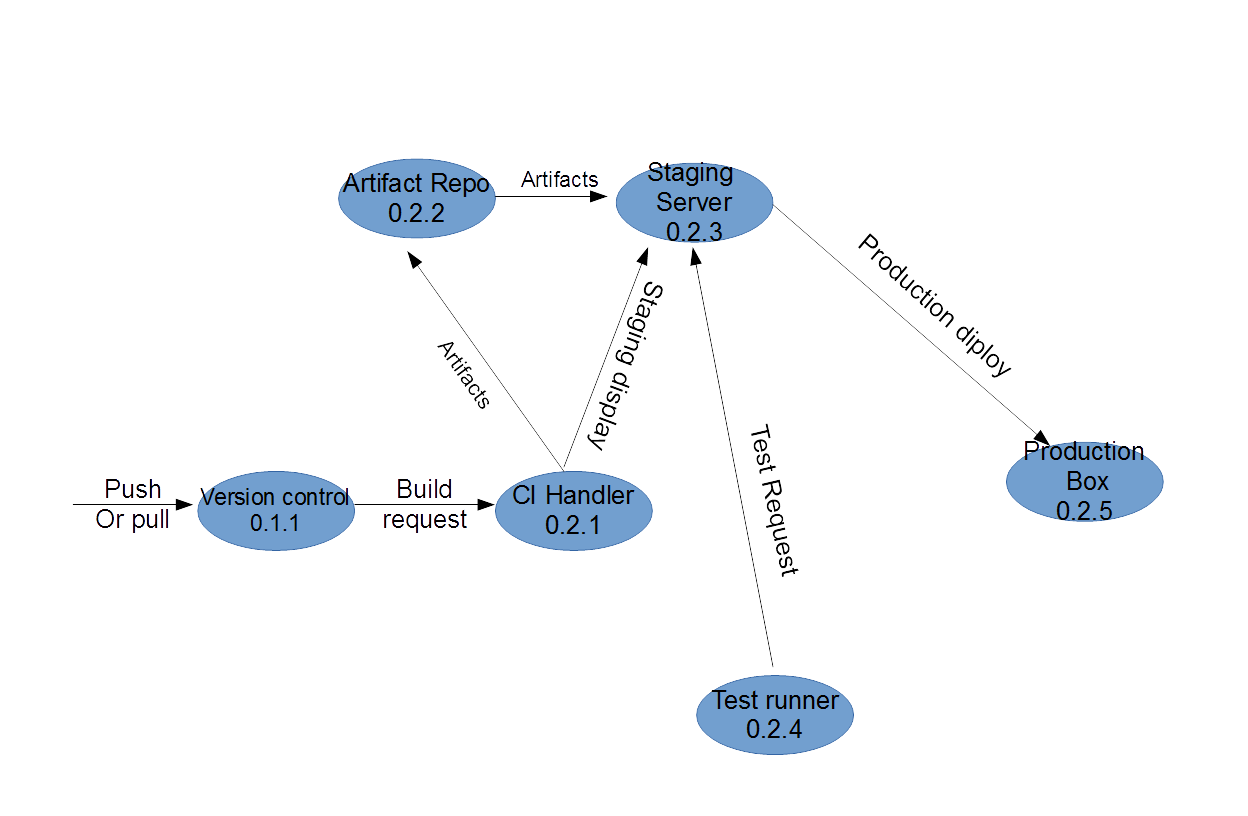
\includegraphics[scale=0.28]{dfd3.png}
\caption{level 2 dfd}
\end{center}
\end{figure}
\end{frame}

\begin{frame}{Flow Diagram}

\begin{figure}[h]
\begin{center}
%\epsfig{width=6in, file=gant.jpg}
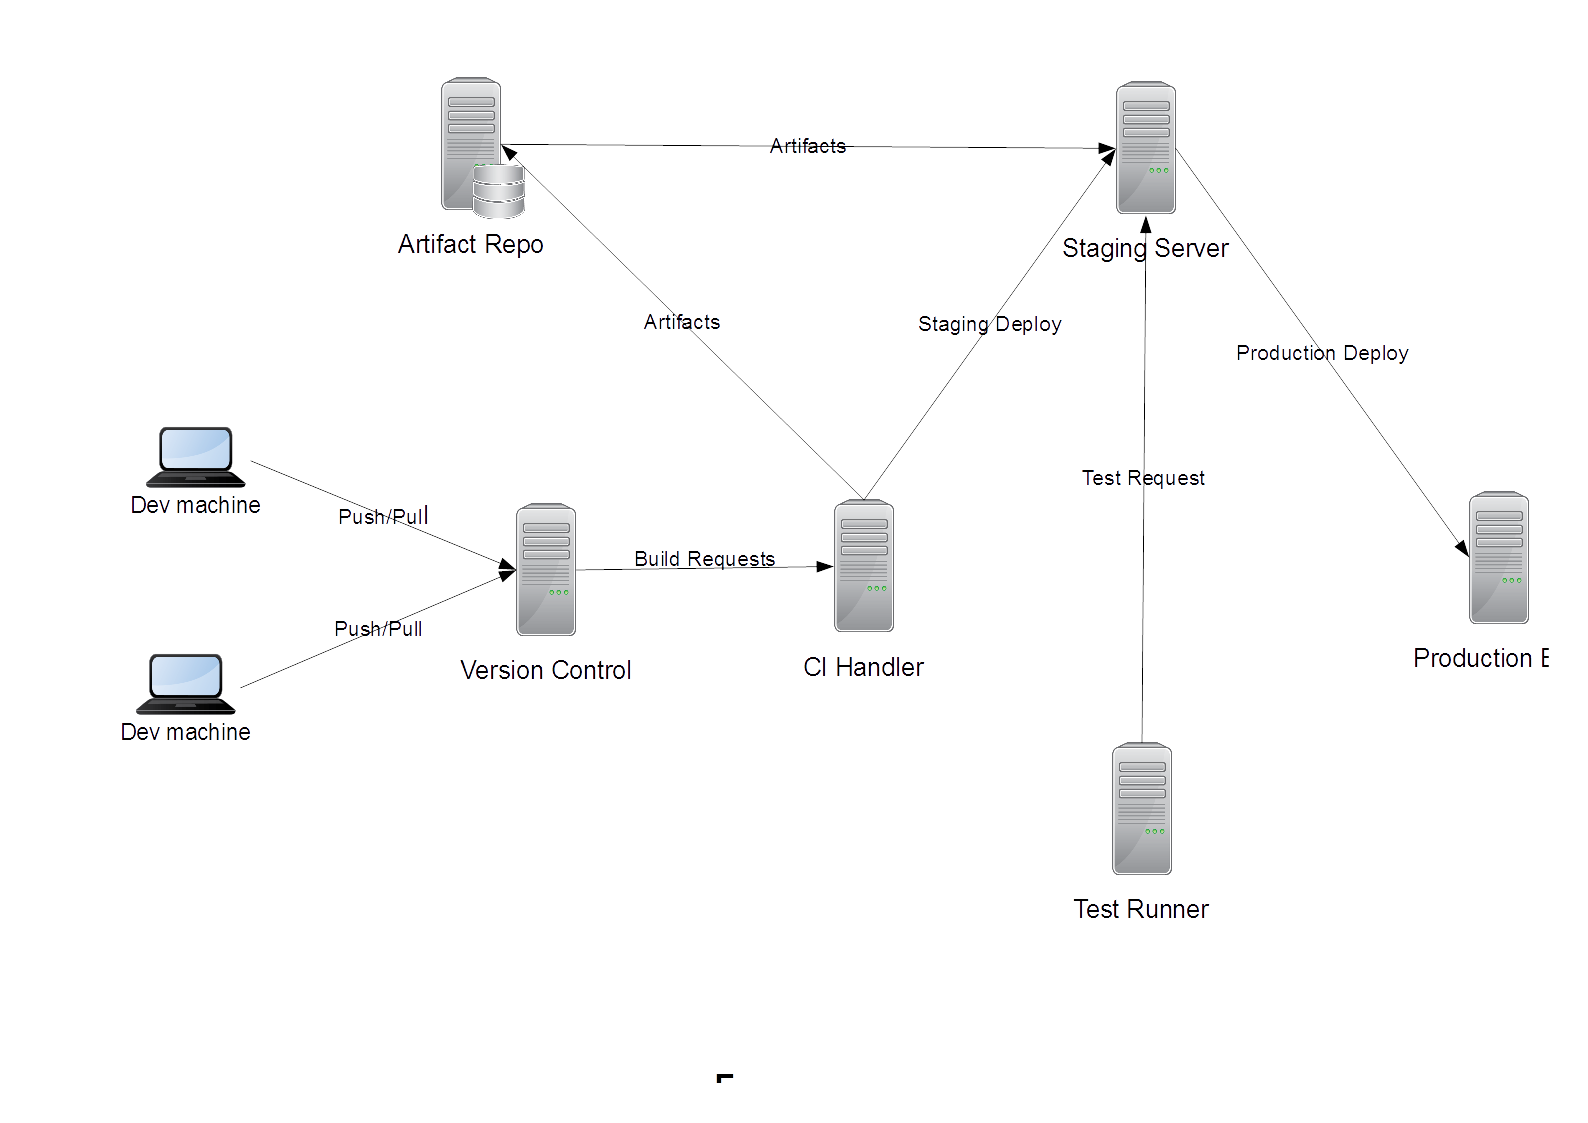
\includegraphics[scale=0.28]{flow1.png}
\caption{Flow Diagram}
\end{center}
\end{figure}
\end{frame}

\begin{frame}{CI Pipeline Diagram}

\begin{figure}[h]
\begin{center}
%\epsfig{width=6in, file=gant.jpg}
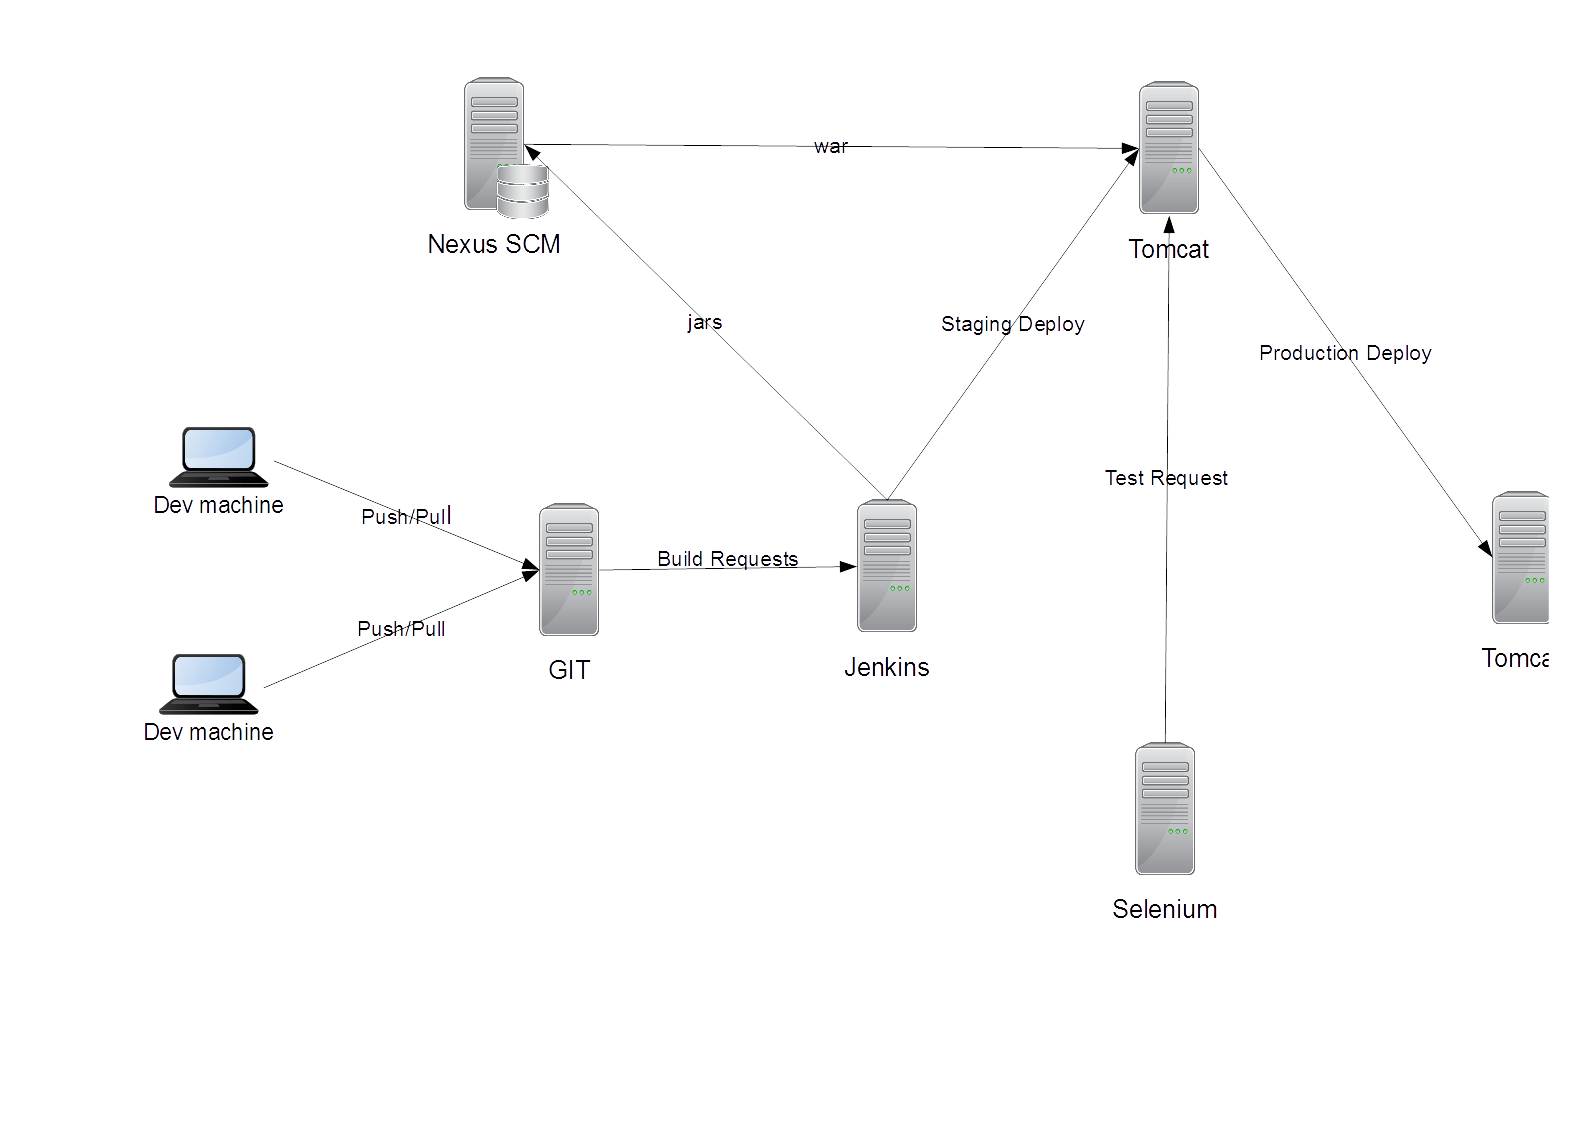
\includegraphics[scale=0.25]{pipeline.png}
\caption{CI Pipeline}
\end{center}
\end{figure}
\end{frame}

\begin{frame}{Sequence Diagram}

\begin{figure}[h]
\begin{center}
%\epsfig{width=6in, file=gant.jpg}
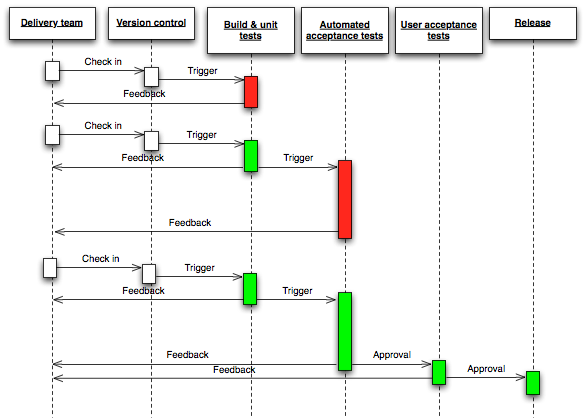
\includegraphics[scale=0.5]{sequence.png}
\caption{Sequence Diagram}
\end{center}
\end{figure}
\end{frame}

\section{IMPLEMENTATION}

\begin{frame}{Implementation}

\begin{itemize}
	\item For demonstration to the Tech 11 Software Team, We decided to implement a Calculator application (using Java, javaScript, NodeJs, Angular...)
	\item We divide the work
	\\
	\begin{itemize}
		\item Addition Module - Vishnu Bose
		\item Subtraction Module - Nitin Suresh
		\item Multiplication Module - Aswin G Sugu
		 \item Division Module - Jeffin Jacob
		 \item View - All
	\end{itemize}
\end{itemize}	
\end{frame}



\begin{frame}{Implementation}
	\textbf{For Version Control}
	\begin{itemize}
		\item Created a Repository named LogicBaker in Git-Hub and cloned to individual systems.
		\item Create module given to each members in java
		\item After Coding the individual modules the team members commit to Git-Hub, irrespective on the platform which each one has build.
		
		 
	
	\end{itemize}	
\end{frame}

\begin{frame}{Implementation}
	\textbf{Artifact Repository}
	\begin{itemize}
		\item An artifact repository is akin to what Subversion is to source code, i.e. it is a way of versifying code binary artifacts. In the Java world these artifacts could be jars, wars, ears, fully fledged applications, libraries or a collections of libraries that are packaged.
				
		
	\end{itemize}	
\end{frame}

\begin{frame}{Implementation}
	\textbf{Artifact Repository}
	\begin{itemize}
		\item The Difficulty in integrating the individual modules due to the syntax mis-matching is overcomed by 
	    Mavenising the Individual modules.
		
		
	\end{itemize}	
\end{frame}






\begin{frame}{Implementation}
	\textbf{Artifact Repository}
	\begin{itemize}
		
		%	a Yiddish word meaning accumulator of knowledge,
		
		
		
		\item Maven was originally started as an attempt to simplify the build processes in the Jakarta Turbine project. There were several projects each with their own Ant build files that were all slightly different and JARs were checked into CVS. We wanted a standard way to build the projects, a clear definition of what the project consisted of, an easy way to publish project information and a way to share JARs across several projects.
		
	\end{itemize}	
\end{frame}


\begin{frame}{Implementation}
	\textbf{Artifact Repository}
	\begin{itemize}
		
		\item The Same Calculator Test application code is mavenised by each team members and again pushed to the local repository.
		\vspace{0.05cm}
		\item The whole can integrated and build in each team members local system mush \underline{easier}. 
		\vspace{0.05cm}
		\item With listed dependencies docs.
	\end{itemize}	
\end{frame}

\begin{frame}{Implementation}
	\textbf{Continous Integration Handler}
	\begin{itemize}
		
		\item To review intermediately the generated code, Understanding what or How it looks like when Deployed?
		\vspace{0.05cm}
		\item Thats the idea behind Continuous Integration, We provide a Automation platform when all team members and the project manager can VIEW the application and discuss.
		  
		
	\end{itemize}	
\end{frame}


\begin{frame}{Implementation}
	\textbf{Continous Integration Handler}
	\begin{itemize}
		
		\item For Automation we use Jenkins.
		\vspace{0.05cm}
		
		\item Jenkins is an open source automation server written in Java. The project was forked from Hudson after a dispute with Oracle. ... It is a server-based system running in a servlet container such as Apache Tomcat.
		
		
	\end{itemize}	
\end{frame}


\begin{frame}{Implementation}
	\textbf{Test Automator}
	\begin{itemize}
		
		\item The test Automation plugging is added to Jenkins depending upon the Nature of the developemnet process dealing with.
		\vspace{0.05cm}
		
		\item which involve programming framework, language etc.
		\vspace{0.05cm}
		\item Since we use Java , we use find-bugs and Check style in Jenkins..
		\vspace{0.05cm}
		\item also added Jacoco , For Cost Estimation.
		
		
	\end{itemize}	
\end{frame}

\section{CONCLUSION}
\begin{frame}{CONCLUSION}
\begin{itemize}
\vspace{10pt}
\item  \textbf{Continually integrate and test to reduce risk.}
\vspace{10pt}
\item  \textbf{Detect problems early.}
\vspace{10pt}
\item  \textbf{Always have a deployable build.}
\vspace{10pt}
\item  \textbf{Generate metrics to guide project management.}
\vspace{10pt}
\item   \textbf{Continuous Integration is:}
\begin{itemize}
\vspace{10pt}
\item \textit{A good practice in any software development method.}
\vspace{10pt}
\item \textit{Vital for agile development.}
\end{itemize}
\end{itemize}
\end{frame}





%------------------------------------------------



%----------------------------------------------------------------------------------------

\end{document} 